\documentclass[14pt,fleqn]{extarticle}
\usepackage[T2A,T1]{fontenc}
\usepackage[utf8]{inputenc}
\usepackage[russian]{babel}
\usepackage{amsmath}
\usepackage{graphicx}
\usepackage{tabularx}
\usepackage{boldline}
\usepackage{makecell}
\usepackage{arydshln}
\usepackage{mathtools}
\usepackage{enumitem}
\usepackage[a4paper, total={6.5in, 9.5in}]{geometry}

\graphicspath{ {./images/} }
\setlength{\mathindent}{0pt}
\setlength\parindent{0pt}


\begin{document}
	\begin{titlepage}
		
\includegraphics[scale=0.12]{logo}
		\begin{center}
			\textbf{МИНОБРНАУКИ РОССИИ}\\
			\vspace{0.2cm}
			\textbf{Федеральное государственное бюджетное образовательное учреждение высшего образования}\\
			\textbf{«САНКТ-ПЕТЕРБУРГСКИЙ ГОСУДАРСТВЕННЫЙ ЭКОНОМИЧЕСКИЙ УНИВЕРСИТЕТ»}\\
			\vspace{0.6cm}
			Факультет информатики и прикладной математики\\
			Кафедра прикладной математики и экономико-математических методов\\
			\vspace{1cm}
			\textbf{ОТЧЁТ}\\
			по дисциплине:\\
			\textbf{«Теория и системы поддержки принятия решений»}\\
			на тему:\\
			\textbf{«Многокритериальная оптимизации на конечном множестве альтернатив. Задание 2»}\\
		\end{center}
		\vspace{1cm}
		Направление: 01.03.02\\
		Обучающийся: Бронников Егор Игоревич\\
		Группа: ПМ-1901\\
		\vfill
		\begin{center}
			Санкт-Петербург\\
			2022\\
		\end{center}
	\end{titlepage}
	
	\section*{Задача 6}
	\textit{Задание:} Задать критерий для каждого пункта, указанного в заголовке таблицы, и упорядочить банки в соответствии с принятыми критериями (тестами)\\
	
	Из всех факторов (признаков) было решено оставить 10 субъективновыбранных:
	\begin{enumerate}[nolistsep]
		\item Максимальная ставка по кредиту, \% $-$ P1 $\leq$ 11.5
		\item Первый взнос, \% $-$ P2 $\leq$ 10
		\item Комиссия банка, \% $-$ P3 $\leq$ 2
		\item Рассмотрение заявки, дн. $-$ P4 $\leq$ 10
		\item Максимальная сумма кредита, млн. руб $-$ P5 $\geq$ 13
		\item Средняя ставка по кредиту, \% $-$ P6 $\leq$ 10
		\item Плата за просрочку, \% $-$ P7 $\leq$ 0.75
		\item Максимальный возраст заёмщика, г. $-$ P8 $\geq$ 60
		\item Максимальный срок кредита, г. $-$ P9 $\geq$ 25
		\item Минимальный общий стаж, г. $-$ P10 $\leq$ 1
	\end{enumerate}
	\begin{center}
		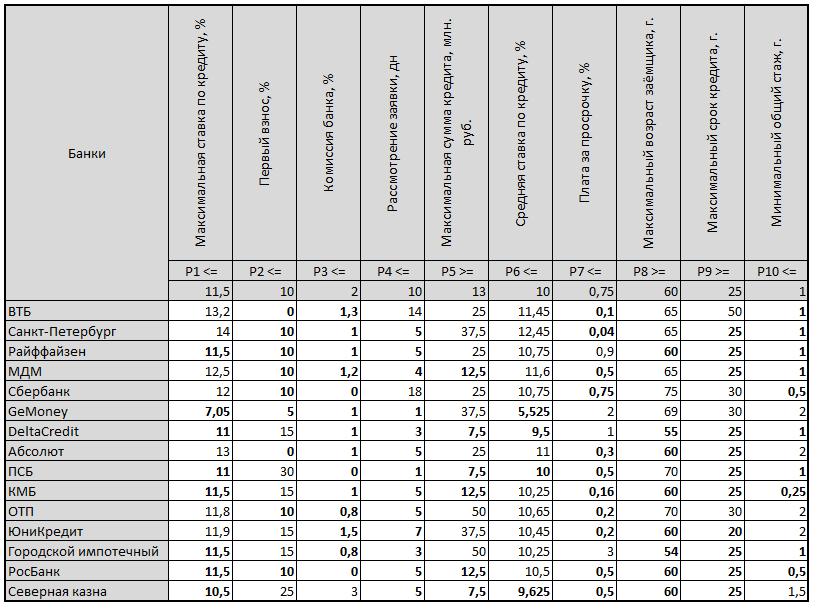
\includegraphics[scale=0.76]{1}
	\end{center}
	\begin{center}
		\textit{Таблица 1} $-$ Характеристики банков
	\end{center}
	\newpage
	Значения признаков, удовлетворяющие ограничениям, выделены полужирным шрифтом. Заменив эти значения единицами, а значения, не удовлетворяющие ограничениям $-$ нулями, получим двоичную таблицу, отражающую выполеннеи заданных ограничений.
	\begin{center}
		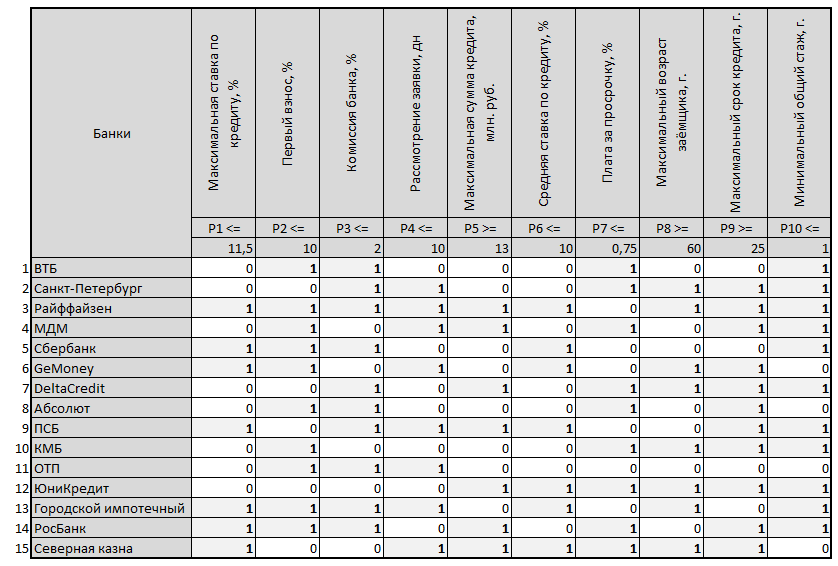
\includegraphics[scale=0.82]{2}
	\end{center}
	\begin{center}
		\textit{Таблица 2} $-$ Оценка свойств банков
	\end{center}
	Воспользуемся оценочной функцией $w_j$ для определения очерёдности критериев в дереве решений:
	\begin{center}
		$w_j = \smashoperator[r]{\sum_{s = 1}^{k_j}}n^0_s n^1_s, \hspace*{1cm} j=\overline{1,n}$
	\end{center}
	, где $n^0_s$ и $n^1_s$ $-$ число нулей и число единиц в $s$-м подмножестве $j$-го уровня, а $k_j$ $-$ число подмножеств на $j$-м уровне.\\
	Результаты вычислений сведены в таблице 3.
	\newpage
	\begin{center}
		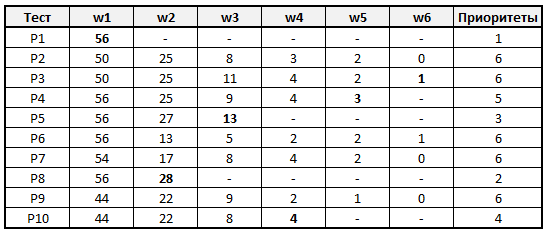
\includegraphics[scale=0.9]{3}
	\end{center}
	\begin{center}
		\textit{Таблица 3} $-$ Определение порядка тестов
	\end{center}
	На основании определения порядка тестов можно построить дерево решений. (\textit{Рисунок 1})
	\begin{center}
		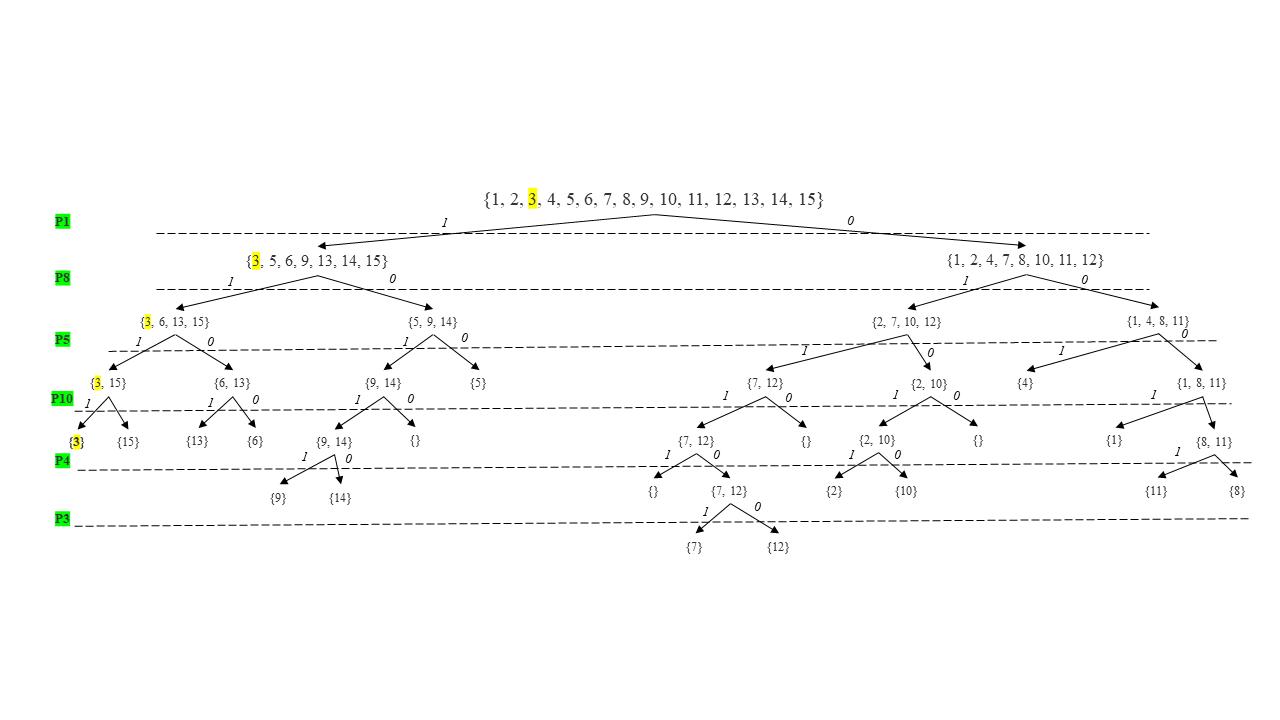
\includegraphics[scale=0.54]{4}
	\end{center}
	\begin{center}
		\textit{Рисунок 1} $-$ Дерево выбора банка
	\end{center}
	Если мы будем идти по левой ветви дерева, то банк который нас удовлетворяет $-$ Райффайзен \{3\}.
	Также данную задачу можно было бы решить и без построения дерева решений. Для этого достаточно в \textit{таблице 3} найти строку с наимбольшим количеством единиц, что означает выполнение максимально возможного количества требований. (\textit{Таблица 4})
	\newpage
	\begin{center}
		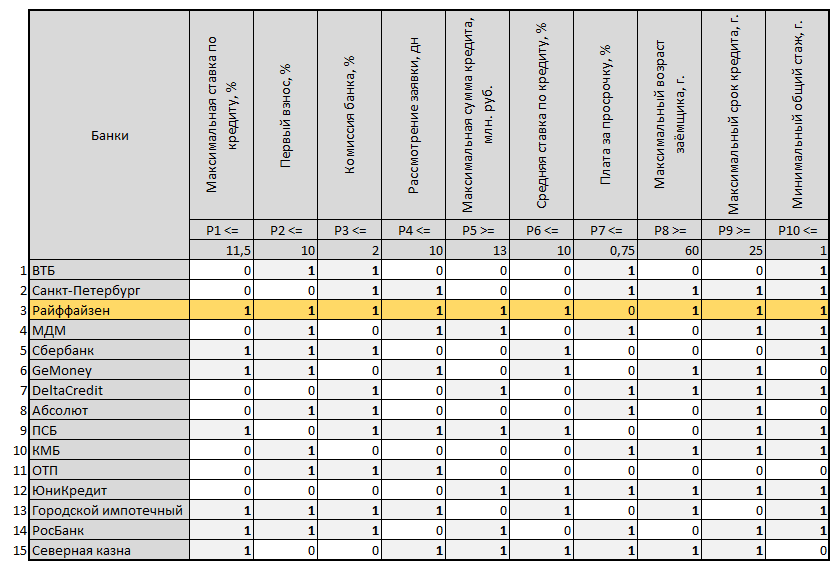
\includegraphics[scale=0.54]{5}
	\end{center}
	\begin{center}
		\textit{Таблица 4} $-$ Выбор банка без дерева решений
	\end{center}
	Если же упорядочивать банки, то мы получим следующий список:
	\begin{enumerate}[nolistsep]
		\item Райффайзен (3)
		\item Северная казна (15)
		\item Городской ипотечный (13)
		\item GeMoney (6)
		\item ПСБ (9)
		\item РосБанк (14)
		\item Сбербанк (5)
		\item DeltaCredit (7)
		\item ЮниКредит (12)
		\item Санкт-Петербург (2)
		\item КМБ (10)
		\item МДМ (4)
		\item ВТБ (1)
		\item ОТП (11)
		\item Абсолют (8)
	\end{enumerate}
	\newpage
	\section*{Задача 7}
	\textit{Задание:} Упорядочить банки по Парето\\
	
	Из всех факторов (признаков) было решено оставить 8 субъективновыбранных:
	\begin{enumerate}[nolistsep]
		\item Максимальная ставка по кредиту, \% $-$ P1 (\textit{min})
		\item Первый взнос, \% $-$ P2 (\textit{max})
		\item Комиссия банка, \% $-$ P3 (\textit{min})
		\item Рассмотрение заявки, дн. $-$ P4 (\textit{min})
		\item Максимальная сумма кредита, млн. руб $-$ P5 (\textit{max})
		\item Средняя ставка по кредиту, \% $-$ P6 (\textit{min})
		\item Максимальный возраст заёмщика, г. $-$ P8 (\textit{min})
		\item Минимальный общий стаж, г. $-$ P10 (\textit{min})
	\end{enumerate}
	\begin{center}
		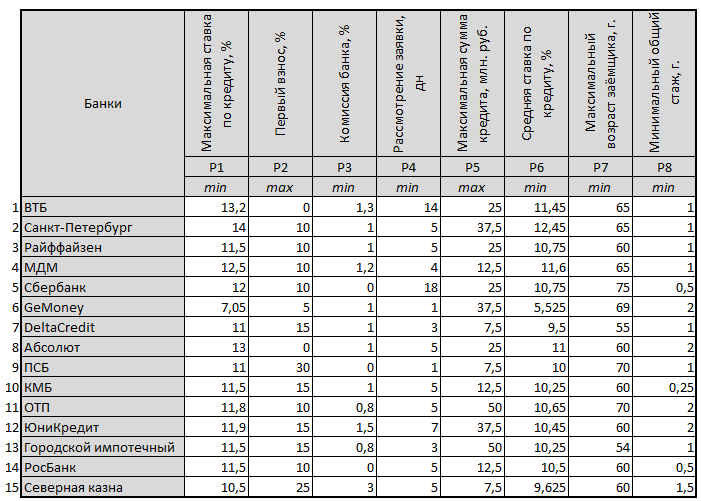
\includegraphics[scale=0.9]{7}
	\end{center}
	\begin{center}
		\textit{Таблица 5} $-$ Характеристики банков
	\end{center}
	\newpage
	Строим матрицу факторов предпочтений. Она представляет собой отношение Парето-доминирования:
	\begin{center}
		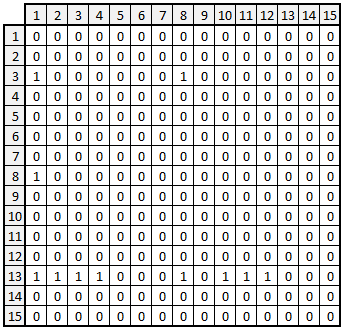
\includegraphics[scale=0.9]{8}
	\end{center}
	\begin{center}
		\textit{Таблица 6} $-$ Матрица факторов предпочтений
	\end{center}
	Название  банков заменены их номерами.\\
	Упорядочив вершины графа от вершин-истоков к вершине-стоку, получим трёхуровневый граф доминирования.\\
	В множество Парето, соответствующее верхнему уровню графа, вошёл только <<Городской ипотечный>> банк.
	\begin{center}
		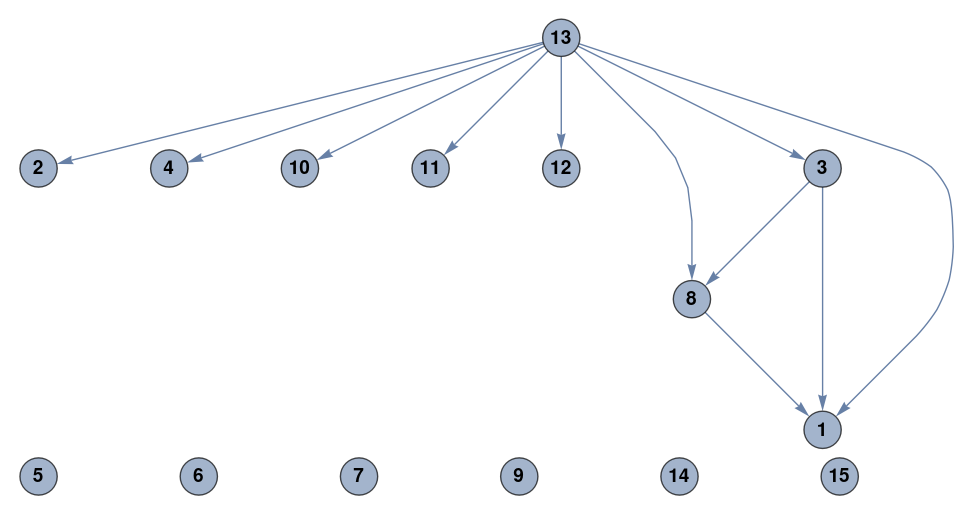
\includegraphics[scale=0.55]{plot}
	\end{center}
	\begin{center}
		\textit{Рисунок 2} $-$ Граф Парето-доминирования, построенный по таблице 6
	\end{center}
	\newpage
	Отношение Парето-доминирования позволяет получить частичный порядок на множестве объектов, поскольку не все объекты сравнимы по Парето.\\
	
	Если же упорядочивать банки, то мы получим следующий список:
	\begin{enumerate}[nolistsep]
		\item Городской ипотечный (13)
		\item Санкт-Петербург (2), МДМ (4), КМБ (10), ОТП (11), ЮниКредит (12), Райффайзен (3), Абсолют (8), ВТБ (1)
		\item Сбербанк (5), GeMoney (6), DeltaCredit (7), ПСБ (9), РосБанк (14), Северная казна (15)
	\end{enumerate}
	
	\subsection*{Показатели отношения Парето-доминирования}

	\subsubsection*{Показатель доминирования}
	Свойство доминирования оценивается числом дуг $m_\textup{д}$, соединяющих вершины верхних уровней ранжированного графа с вершинами нижних уровней. Отсюда \textit{показатель доминирования} $k_\textup{д}$ вычисляется как доля дуг в общем числе связей полного графа:
	\begin{center}
		$k_\textup{д} = \dfrac{2 \cdot m_\textup{д}}{N(N-1)}$
	\end{center}

	\begin{center}
		$k_\textup{д} = \dfrac{2 \cdot 8}{15(15-1)} = 0.0761905 = 7.61905\%$
	\end{center}

	\subsubsection*{Показатель неразличимости объектов}
	\textit{Неразличимость объектов} количественно оцениваются числом рёбер $m_\textup{р}$, соединяющих вершины, принадлежащие одному уровню графа, и оценивается формулой:
	\begin{center}
		$k_\textup{нр} = \dfrac{2 \cdot m_\textup{р}}{N(N-1)}$
	\end{center}
	
	\begin{center}
		$k_\textup{нр} = \dfrac{2 \cdot 3}{15(15-1)} = 0.0285714 = 2.85714\%$
	\end{center}

	\subsubsection*{Показатель несравнимости объектов}
	Число отсутствующих связей, характеризующее долю \textit{несравнимых объектов}, вычисляется по формуле:
	
	\begin{center}
		$k_\textup{нс} = 1 - (k_\textup{д} + k_\textup{нр})$
	\end{center}

	\newpage
	
	\begin{center}
		$k_\textup{нс} = 1 - (0.0761905 + 0.0285714) = 0.895238 = 89.5238\%$
	\end{center}

	\subsubsection*{Показатель строгости порядка}
	Показатель \textit{строгости порядка} $k_\textup{сп}$ определим как отношение числа уровней графа к числу объектов:
	
	\begin{center}
		$k_\textup{сп} = \dfrac{\rho_{max} - 1}{N-1}$
	\end{center}

	\begin{center}
		$k_\textup{сп} = \dfrac{3-1}{15-1} = 0.142857 = 14.2857\%$
	\end{center}

	\subsubsection*{Расчёт полустепеней захода и исхода}
	Полустепень захода ($deg^+(x_i)$) -- число дуг, заходящих в вершину $x_i$\\
	Полустепень исхода ($deg^-(x_i)$) -- число дуг, исходящих из вершины $x_i$\\
	
	$\rho_{max}(x_i)$ -- лучший ранг вершины $x_i$ с полустепенью захода $deg^-(x_i)$
	\begin{center}
		$\rho_{max}(x_i) = N - deg^-(x_i)$
	\end{center}
	$\rho_{min}(x_i)$ -- лучший ранг вершины $x_i$ с полустепенью исхода $deg^+(x_i)$
	\begin{center}
		$\rho_{min}(x_i) = deg^+(x_i) + 1$
	\end{center}

	\textit{Расчёты:}
	
	$deg^+(1) = 3$ \hspace{0.55cm} $deg^-(1) = 0$ \hspace{0.55cm} $\rho_{min}(1) = 4$ \hspace{0.55cm} $\rho_{max}(1) = 15$

	$deg^+(2) = 1$ \hspace{0.55cm} $deg^-(2) = 0$ \hspace{0.55cm} $\rho_{min}(2) = 2$ \hspace{0.55cm} $\rho_{max}(2) = 15$
	
	$deg^+(3) = 1$ \hspace{0.55cm} $deg^-(3) = 2$ \hspace{0.55cm} $\rho_{min}(3) = 2$ \hspace{0.55cm} $\rho_{max}(3) = 13$
	
	$deg^+(4) = 1$ \hspace{0.55cm} $deg^-(4) = 0$ \hspace{0.55cm} $\rho_{min}(4) = 2$ \hspace{0.55cm} $\rho_{max}(4) = 15$
	
	$deg^+(5) = 0$ \hspace{0.55cm} $deg^-(5) = 0$ \hspace{0.55cm} $\rho_{min}(5) = 1$ \hspace{0.55cm} $\rho_{max}(5) = 15$
	
	$deg^+(6) = 0$ \hspace{0.55cm} $deg^-(6) = 0$ \hspace{0.55cm} $\rho_{min}(6) = 1$ \hspace{0.55cm} $\rho_{max}(6) = 15$
	
	$deg^+(7) = 0$ \hspace{0.55cm} $deg^-(7) = 0$ \hspace{0.55cm} $\rho_{min}(7) = 1$ \hspace{0.55cm} $\rho_{max}(7) = 15$
	
	$deg^+(8) = 2$ \hspace{0.55cm} $deg^-(8) = 1$ \hspace{0.55cm} $\rho_{min}(8) = 3$ \hspace{0.55cm} $\rho_{max}(7) = 14$

	$deg^+(9) = 0$ \hspace{0.55cm} $deg^-(9) = 0$ \hspace{0.55cm} $\rho_{min}(9) = 1$ \hspace{0.55cm} $\rho_{max}(9) = 15$
	
	$deg^+(10) = 1$ \hspace{0.3cm} $deg^-(10) = 0$ \hspace{0.3cm} $\rho_{min}(10) = 2$ \hspace{0.3cm} $\rho_{max}(10) = 15$
	
	$deg^+(11) = 1$ \hspace{0.3cm} $deg^-(11) = 0$ \hspace{0.3cm} $\rho_{min}(11) = 2$ \hspace{0.3cm} $\rho_{max}(11) = 15$
	
	$deg^+(12) = 1$ \hspace{0.3cm} $deg^-(12) = 0$ \hspace{0.3cm} $\rho_{min}(12) = 2$ \hspace{0.3cm} $\rho_{max}(12) = 15$

	$deg^+(13) = 0$ \hspace{0.3cm} $deg^-(13) = 8$ \hspace{0.3cm} $\rho_{min}(13) = 1$ \hspace{0.3cm} $\rho_{max}(13) = 7$
	
	$deg^+(14) = 0$ \hspace{0.3cm} $deg^-(14) = 0$ \hspace{0.3cm} $\rho_{min}(14) = 1$ \hspace{0.3cm} $\rho_{max}(14) = 15$

	$deg^+(15) = 0$ \hspace{0.3cm} $deg^-(15) = 0$ \hspace{0.3cm} $\rho_{min}(15) = 1$ \hspace{0.3cm} $\rho_{max}(15) = 15$\\

	Таким образом, мы получили информацию о границах упорядочения объектов.
	
	\newpage
	\section*{Задача 8}
	\textit{Задание:} Расположить критерии по важности и упорядочить банки в соответствие с их лексикографическим порядком. Затем рассмотреть критерии в обратном порядке и упорядочить банки в соответствие с их новым лексикографическим порядком\\
	
	Из всех факторов (признаков) было решено оставить 8 субъективновыбранных:
	\begin{enumerate}[nolistsep]
		\item Максимальная ставка по кредиту, \% $-$ P1 (\textit{min})
		\item Первый взнос, \% $-$ P2 (\textit{max})
		\item Комиссия банка, \% $-$ P3 (\textit{min})
		\item Рассмотрение заявки, дн. $-$ P4 (\textit{min})
		\item Максимальная сумма кредита, млн. руб $-$ P5 (\textit{max})
		\item Средняя ставка по кредиту, \% $-$ P6 (\textit{min})
		\item Максимальный возраст заёмщика, г. $-$ P8 (\textit{min})
		\item Минимальный общий стаж, г. $-$ P10 (\textit{min})
	\end{enumerate}

	\subsection*{Прямой порядок}
	Приоритет критериев берём из условия.
	\begin{center}
		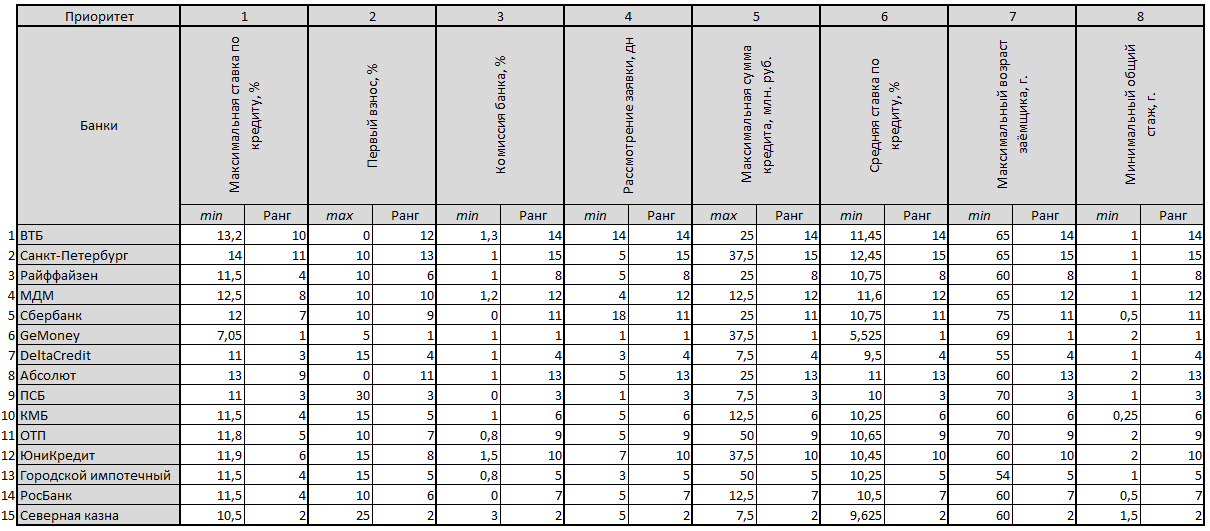
\includegraphics[scale=0.55]{9}
	\end{center}
	\begin{center}
		\textit{Таблица 7} $-$ Характеристики банков в обычной и ранговой шкале
	\end{center}
	Получается, что после третьего критерия мы получили успорядоченный список банков.\\
	\newpage
	Упорядоченный список банков:
	\begin{enumerate}[nolistsep]
		\item GeMoney (6)
		\item Северная казна (15)
		\item ПСБ (9)
		\item DeltaCredit (7)
		\item Городской ипотечный (13)
		\item КМБ (10)
		\item РосБанк (14)
		\item Райффайзен (3)
		\item ОТП (11)
		\item ЮниКредит (12)
		\item Сбербанк (5)
		\item МДМ (4)
		\item Абсолют (8)
		\item ВТБ (1)
		\item Санкт-Петербург (2)
	\end{enumerate}

	\subsection*{Обратный порядок}
	Приоритет критериев берём из перевёрнутого списка условий.
	\begin{center}
		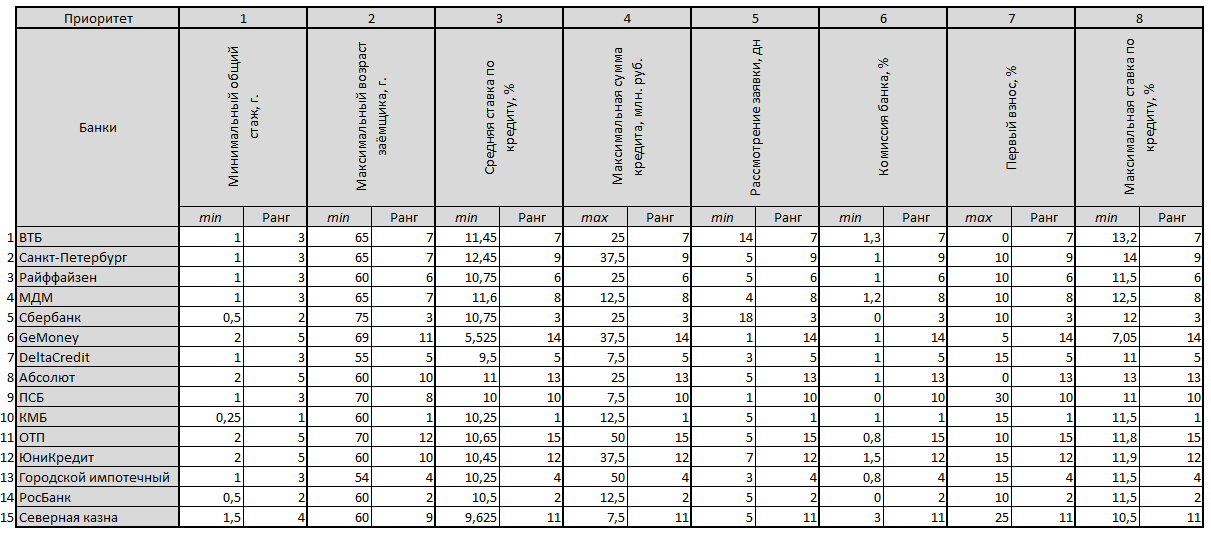
\includegraphics[scale=0.55]{10}
	\end{center}
	\begin{center}
		\textit{Таблица 8} $-$ Характеристики банков в обычной и ранговой шкале
	\end{center}
	Получается, что после третьего критерия мы получили успорядоченный список банков.\\
	\newpage
	Упорядоченный список банков:
	\begin{enumerate}[nolistsep]
		\item КМБ (10)
		\item РосБанк (14)
		\item Сбербанк (5)
		\item Городской ипотечный (13)
		\item DeltaCredit (7)
		\item Райффайзен (3)
		\item ВТБ (1)
		\item МДМ (4)
		\item Санкт-Петербург (2)
		\item ПСБ (9)
		\item Северная казна (15)
		\item ЮниКредит (12)
		\item Абсолют (8)
		\item GeMoney (6)
		\item ОТП (11)
	\end{enumerate}
\end{document}